% Railway Digital Twin with Wildlife Safety — compact 10-page report
% College of Engineering, Guindy — Anna University, Chennai - 25
% Embedded Systems and Internet of Things — Team 14
\documentclass[10pt,a4paper,twocolumn]{article}

\usepackage[a4paper,margin=1.5cm,columnsep=0.7cm,top=1.4cm,bottom=1.6cm]{geometry}
\usepackage[T1]{fontenc}
\usepackage[utf8]{inputenc}
\usepackage{graphicx}
\usepackage{booktabs}
\usepackage{tabularx}
\usepackage{array}
\usepackage{enumitem}
\usepackage{xcolor}
\usepackage{float}
\usepackage{amsmath}
\usepackage{caption}
\usepackage[hidelinks]{hyperref}
\usepackage{url}

\graphicspath{{figures/}}
\setlength{\parindent}{0pt}
\setlength{\parskip}{2.5pt}
\captionsetup{font=scriptsize,labelfont=bf,skip=2pt}
\setlist{itemsep=1pt,topsep=2pt,parsep=0pt,leftmargin=*}
\newcommand{\sect}[1]{\section{#1}}

\begin{document}

% ================= PAGE 1: TITLE + TEAM =================
\twocolumn[{%
\begin{center}
{\footnotesize\bfseries COLLEGE OF ENGINEERING, GUINDY --- ANNA UNIVERSITY, CHENNAI -- 25}\\[1pt]
{\footnotesize Course: Embedded Systems and Internet of Things \;$\vert$\; \textbf{Team: 14}}\\[6pt]
{\LARGE\bfseries Railway Digital Twin with Wildlife Safety}\\[2pt]
{\small An educational simulation integrating Godot 4, MQTT, a trusted Node.js control plane, React dashboards and ESP32 edge sensing}\\[6pt]
{\small\textbf{Team members:}}\\[2pt]
{\small
\begin{tabular}{rl@{\hspace{18pt}}rl}
\textbf{Roll No.} & \textbf{Name} & \textbf{Roll No.} & \textbf{Name}\\
2023103546 & Kathir Kalidass B & 2023103600 & Parthasarathi S\\
2023103597 & Malini R & 2023103714 & Paril T\\
\end{tabular}}
\end{center}
\vspace{4pt}
}]

\begin{abstract}
\noindent\textbf{Abstract ---} A runnable digital twin of a wildlife-protected railway line: a Godot~4.7 3-D double-track ``stadium'' world with an island station, interlocked crossovers, level crossing, river bridges and Libre-TrainSim-derived asset fleet; a Node.js trusted control plane (JWT, RBAC, envelope validation, SQLite anti-replay and audit) that is the sole publisher of commands/state/signals on an authenticated Mosquitto MQTT broker with per-client ACLs; a React dashboard for viewer/operator/admin; an ESP32 edge node with fail-safe outputs verified in Wokwi over a Pinggy tunnel; and a FastAPI ML service (torchvision SSDLite) behind a two-frame camera-evidence policy. Wildlife protection escalates NONE$\rightarrow$SUSPECTED (30\,km/h)$\rightarrow$CONFIRMED (0\,km/h, STOP/RED) from trackside huts, an onboard simulated camera and ESP32 reports, with recovery-latched resets. Verification: Godot 42/42, backend 141/141, ML 8/8, ESP32 native 16/16, web build PASS, plus recorded live scenarios. Educational simulation only --- not railway safety equipment.
\end{abstract}

% ================= 1. INTRODUCTION =================
\sect{I. Introduction and Objectives}
Train--animal collisions on forested corridors motivate layered protection: \emph{digital twins} let operators observe and rehearse operations while \emph{embedded IoT edge nodes} sense hazards where they occur. Team 14 built a complete, runnable miniature railway covering both ideas. Objectives: (1) a 3-D double-track twin with real interlocking; (2) a trusted, audited, anti-replay control plane; (3) end-to-end security across REST and MQTT; (4) staged wildlife sensing (trackside hut, onboard camera, edge node) with two-frame camera confirmation; (5) an ESP32 fail-safe field node verified in a cloud simulator; (6) role-aware dashboards; (7) a continuous automated test gate. \textbf{Scope:} classroom simulation only; the Stage-D physical-hardware checklist is \emph{not run}.

% ================= 2. ARCHITECTURE =================
\sect{II. Architecture}
One principle: \emph{one trusted control plane, many restricted clients}. The Node backend is the sole MQTT publisher of \texttt{railway/state}, \texttt{events}, \texttt{alerts}, \texttt{signal/\{block\}} (retained), \texttt{commands/*} and \texttt{speed/*}. Mosquitto~2 (TCP 1883, WS 9001) authenticates four clients --- \texttt{backend}, \texttt{godot}, \texttt{dashboard}, \texttt{esp32} --- with generated credentials and per-client topic ACLs (Appendix matrix in the extended version; dashboard is read-only, ESP32 publishes only non-retained telemetry). Backend modules: \texttt{state.js}/\texttt{simulation.js} (two-train fleet: T1 UP clockwise, T3 DOWN anticlockwise; ten blocks), \texttt{signalling.js}/\texttt{routes.js} (per-block aspects, station-crossover interlock), \texttt{meets.js}/\texttt{rng.js} (seeded chance-meet scheduler), \texttt{wrong\_line.js} (interlocked wrong-line run), \texttt{wildlife\_commands.js}/\texttt{ingest.js}/\texttt{ml.js} (evidence fusion and camera ingest), \texttt{auth.js}/\texttt{rbac.js}/\texttt{replay.js}/\texttt{audit.js}/\texttt{db.js} (SQLite-backed security), \texttt{loop.js} (2\,Hz fixed-timestep authority loop), \texttt{bus.js}/\texttt{mqtt.js} (retained publication). Failure posture: restrictive fail-safe on MQTT loss (\texttt{COMM\_LOST}), retained snapshot reconcile on reconnect, recovery latch (\texttt{RECOVERY\_REQUIRED}) until an authorised RESET, and no replay of stale envelopes or telemetry.

\sect{III. Workflow}\label{sec:workflow}
\textbf{Control path (REST):} operator logs in (\texttt{/api/login}, bcrypt + JWT) $\rightarrow$ issues \texttt{/api/control}, \texttt{/api/route}, \texttt{/api/meet}, \texttt{/api/speed}, \texttt{/api/wrong-line} $\rightarrow$ backend validates role, envelope schema, $\pm$5\,min timestamp freshness and replay registry $\rightarrow$ publishes authoritative state (retained, 2\,Hz). \textbf{Observation path (MQTT):} twin/ESP32 telemetry and wildlife evidence $\rightarrow$ backend fuses \emph{trackside} + \emph{onboard} evidence $\rightarrow$ block aspects (SUSPECTED$\rightarrow$YELLOW, CONFIRMED$\rightarrow$RED), alerts, ESP32 commands (\texttt{WILDLIFE\_NEAR}, \texttt{WILDLIFE\_DETECTED}, \texttt{RESET}) $\rightarrow$ dashboard WebSocket and twin reconciler update; ESP32 local inputs always dominate remote commands. Three independent protectors act on the same event: twin local limit (zero-latency braking even with MQTT offline), backend authority, and the edge node's own restrictive outputs. Demo: \texttt{./scripts/dev-up.sh} brings up the stack; \texttt{scripts/demo-scenarios.sh} drives the authenticated flow.

% ================= 4. TOOLS =================
\sect{IV. Tools and Technology}
\begin{table}[H]\scriptsize
\caption{Technology stack}\label{tab:stack}
\begin{tabularx}{\linewidth}{p{1.7cm} X}
\toprule
\textbf{Layer} & \textbf{Technology (version / role)}\\
\midrule
Control plane & Node.js 22+, Express 4.21, better-sqlite3 13 (WAL), bcryptjs 3, jsonwebtoken 9, mqtt.js 5.16; Node built-in test runner (141 tests)\\
Live bus & Eclipse Mosquitto 2: authenticated MQTT, retained topics, per-client ACLs\\
Twin & Godot 4.7.2 (\texttt{gl\_compatibility}; runs headless under \texttt{xvfb-run}); vendored \texttt{godot-mqtt} addon; 42-suite test harness\\
Assets & Blender-exported GLBs from Libre-TrainSim (train consist, station modules, deer/elephant) via \texttt{tools/export\_lts\_assets.py}; \texttt{test\_real\_assets} proves the exports replace procedural stubs\\
Dashboard & React 18.3.1 + Vite 6 + TypeScript 5.7 (\texttt{tsc --noEmit} gate)\\
Edge & PlatformIO espressif32 Arduino: PubSubClient 2.8, ArduinoJson 7, ESP32Servo, Adafruit SSD1306/GFX; Unity native tests\\
Edge sim & Wokwi (\texttt{diagram.json}, \texttt{wokwi.toml}, \texttt{scenarios/wildlife.yaml}, CLI v0.29.0); Pinggy raw-TCP tunnel to the local broker\\
ML & FastAPI 0.135.1 + uvicorn; torchvision 0.25 \texttt{ssdlite320\_mobilenet\_v3\_large}, COCO animal classes; \texttt{ML\_STUB=1} deterministic elephant 0.92 for integration runs\\
DevOps & Docker Compose, \texttt{dev-up.sh}, \texttt{verify-all.sh} gate\\
\bottomrule
\end{tabularx}
\end{table}

% ================= 5. PERIPHERALS =================
\sect{V. Peripherals (ESP32 Edge Node)}
Field peripherals are wired in Wokwi and driven by the production firmware; the decision core lives in six pure-function headers (\texttt{sensors.h}, \texttt{debounce.h}, \texttt{output\_logic.h}, \texttt{actuator.h}, \texttt{telemetry.h}, \texttt{command\_logic.h}) so all logic is host-testable.
\begin{table}[H]\scriptsize
\caption{Peripheral map (from \texttt{esp32/diagram.json}, 29 wires)}\label{tab:periph}
\begin{tabularx}{\linewidth}{p{2.6cm} p{1.55cm} X}
\toprule
\textbf{Peripheral} & \textbf{Pin} & \textbf{Function}\\
\midrule
Green / Red LED & GPIO26 / GPIO25 & CLEAR vs RESTRICTIVE indicator\\
Buzzer & GPIO27 & hazard alarm; \texttt{NEAR} pulsed warning\\
Wildlife button & GPIO33 & field witness: animal at crossing\\
Fault button & GPIO32 & sensor-fault witness; blocks RESET\\
HC-SR04 ultrasonic & GPIO5/18 & obstacle distance (cm$\rightarrow$m)\\
PIR motion & GPIO19 & passive motion detection\\
Vibration (analog) & GPIO34 & vibration threshold input\\
Barrier servo & GPIO13 & boom 0$^\circ$ open / 90$^\circ$ restrictive\\
SSD1306 OLED & I$^2$C 21/22 & status-line display\\
\bottomrule
\end{tabularx}
\end{table}
Sensor fusion: \texttt{animal\_detected} $=$ PIR $\lor$ distance$\le$threshold $\lor$ vibration$\ge$threshold. Output precedence: \texttt{LOCAL WILDLIFE/FAULT} $>$ \texttt{COMM LOSS} $>$ backend stop $>$ \texttt{ANIMAL NEAR} $>$ \texttt{CLEAR} --- local inputs are debounced and can never be cleared remotely. Telemetry carries \texttt{request\_id}, zone, \texttt{device}, \texttt{sensorHealthy}, \texttt{wildlifeDetected}, \texttt{nearAnimal}, \texttt{uptimeMs}, \texttt{distanceM}, \texttt{motion}, \texttt{vibration}; SNTP-gated clock (\texttt{clockValid:false} + null timestamp until valid, which the backend rejects). Reconnect/publish is non-blocking; nothing is queued for replay.

% ================= 6. HARDWARE / SIMULATION =================
\sect{VI. Hardware and Simulation}
The ESP32 path is verified \emph{without physical hardware} in two layers: (i) 16 Unity native cases (output precedence, debounce, telemetry serialization, command-zone validation) via \texttt{pio test -e native}, firmware builds \texttt{esp32dev} (Flash 87.1\%); (ii) Wokwi cloud simulation of the exact \texttt{diagram.json} wiring running the same \texttt{firmware.bin}: \texttt{wokwi-tunnel.sh --write-secrets} opens a Pinggy raw-TCP tunnel and writes device-reachable endpoints into git-ignored \texttt{secrets.h}; \texttt{scenarios/wildlife.yaml} produces serial \texttt{MQTT connected} then \texttt{STATE LOCAL WILDLIFE}, observed live in the twin as \texttt{external=true} STOP/RED with the backend latched \texttt{RECOVERY\_REQUIRED}. Stage-D checklist status: boot-restrictive and wildlife-input rows \textbf{PASS (Wokwi 2026-10-21)}; same/out-of-zone dashboard controls, reconnect behaviour and full serial inspection on physical hardware \textbf{not run}. Host evidence: Linux headless verification with Mesa llvmpipe (and WSLg D3D12 GPU at $\approx$11.8\,ms/frame, 1280$\times$720).

% ================= 7. TWIN + SCREENSHOTS =================
\sect{VII. Digital Twin World and Screenshots}
The twin (\texttt{godot/scenes/lts\_full.tscn}) renders a shared 250\,m straight-sided stadium footprint (UP 1253.9822\,m, DOWN 1228.8495\,m; blocks 250.796/245.77\,m), T1 clockwise and T3 anticlockwise with operational-chainage conversion (Fig.~\ref{fig:ovr}), an island platform spanning 150--198\,m between the tracks inside \texttt{UP-B2}/\texttt{DOWN-B2} (Fig.~\ref{fig:plf}), two interlocked station crossovers (X-A at 120\,m, X-B at 240\,m) used by meets and wrong-line runs (Fig.~\ref{fig:wl}), a two-track wildlife level crossing with boom barriers and alarm, carved river with road + railway bridges, catenary, block signal masts, ten trackside sensor huts (75\,m overlapping radius) and an onboard simulated camera. Keys: \texttt{SPACE} wildlife, \texttt{F} fault, \texttt{R} reset, \texttt{TAB} train switch, \texttt{C} camera, \texttt{N} day/night, \texttt{B} cinematic reel. All figures below were regenerated from \texttt{godot/tests/capture\_*.gd} under headless software rendering (HUD shows \texttt{MQTT offline} in capture mode --- expected).

\begin{figure*}\centering
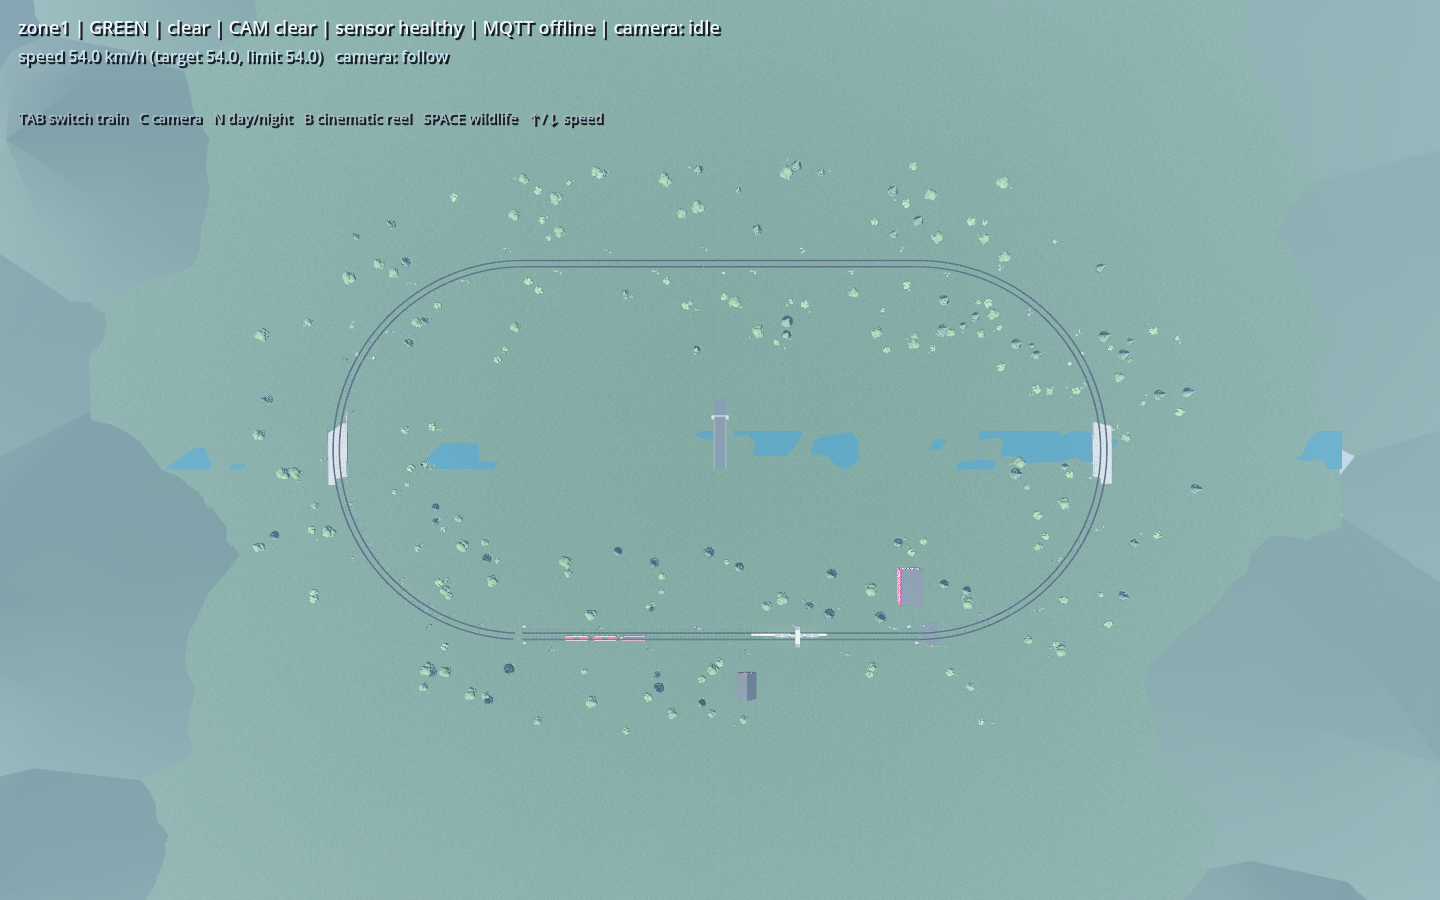
\includegraphics[width=15.2cm]{double_track_overview.png}
\caption{Top-down overview: stadium double track, island station, river with bridges, HUD state bar.}
\label{fig:ovr}
\end{figure*}

\begin{figure*}\centering
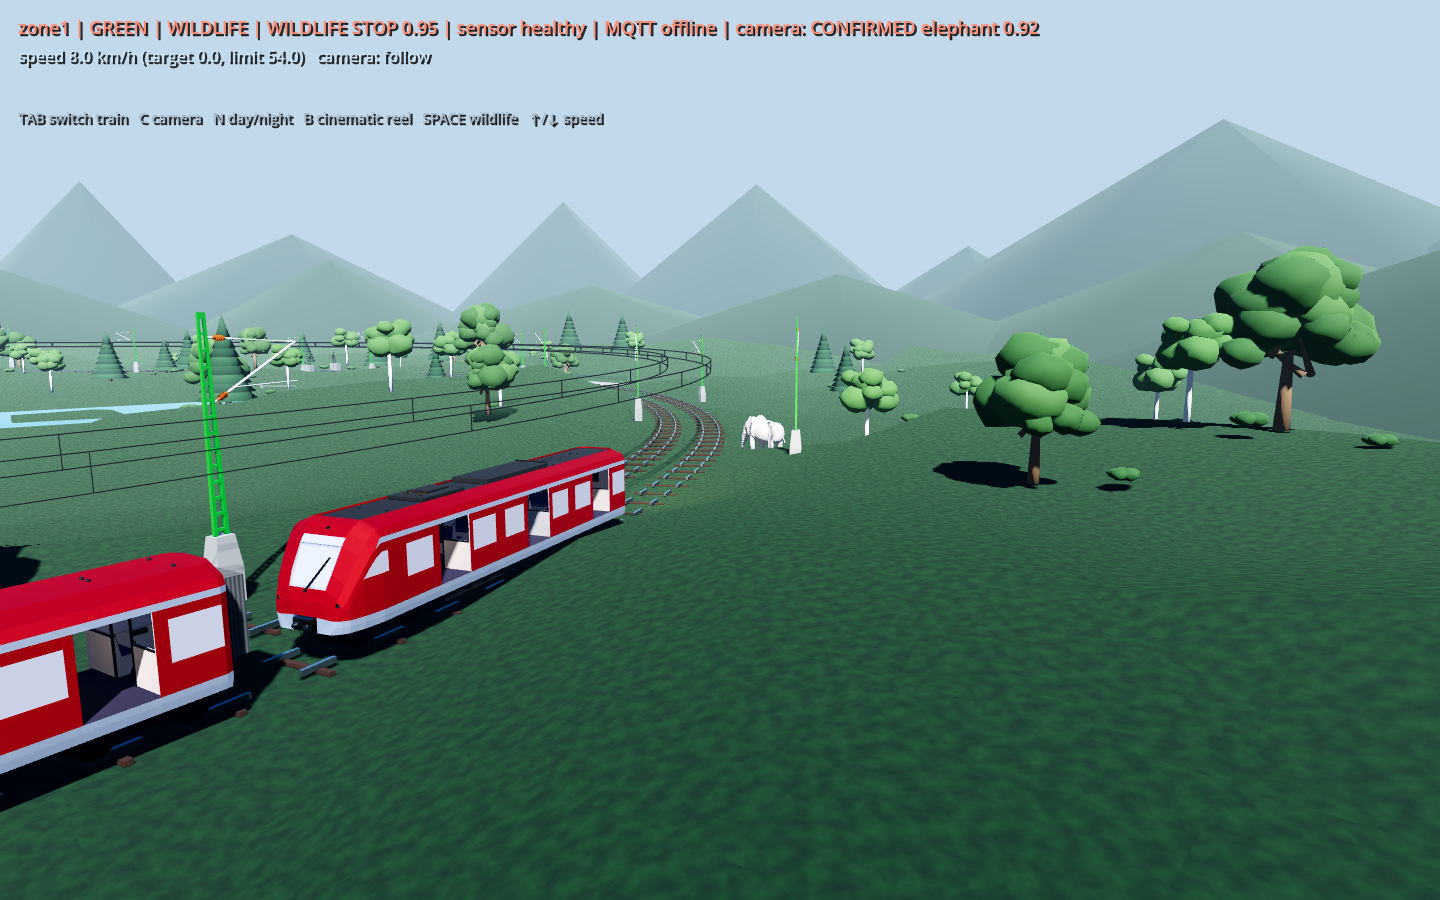
\includegraphics[width=15.2cm]{camera_confirm.png}
\caption{Confirmed wildlife stop: HUD \texttt{WILDLIFE STOP 0.95 / camera: CONFIRMED elephant 0.92}; target 0\,km/h, elephant ahead, barrier down.}
\label{fig:cam}
\end{figure*}

\begin{figure*}\centering
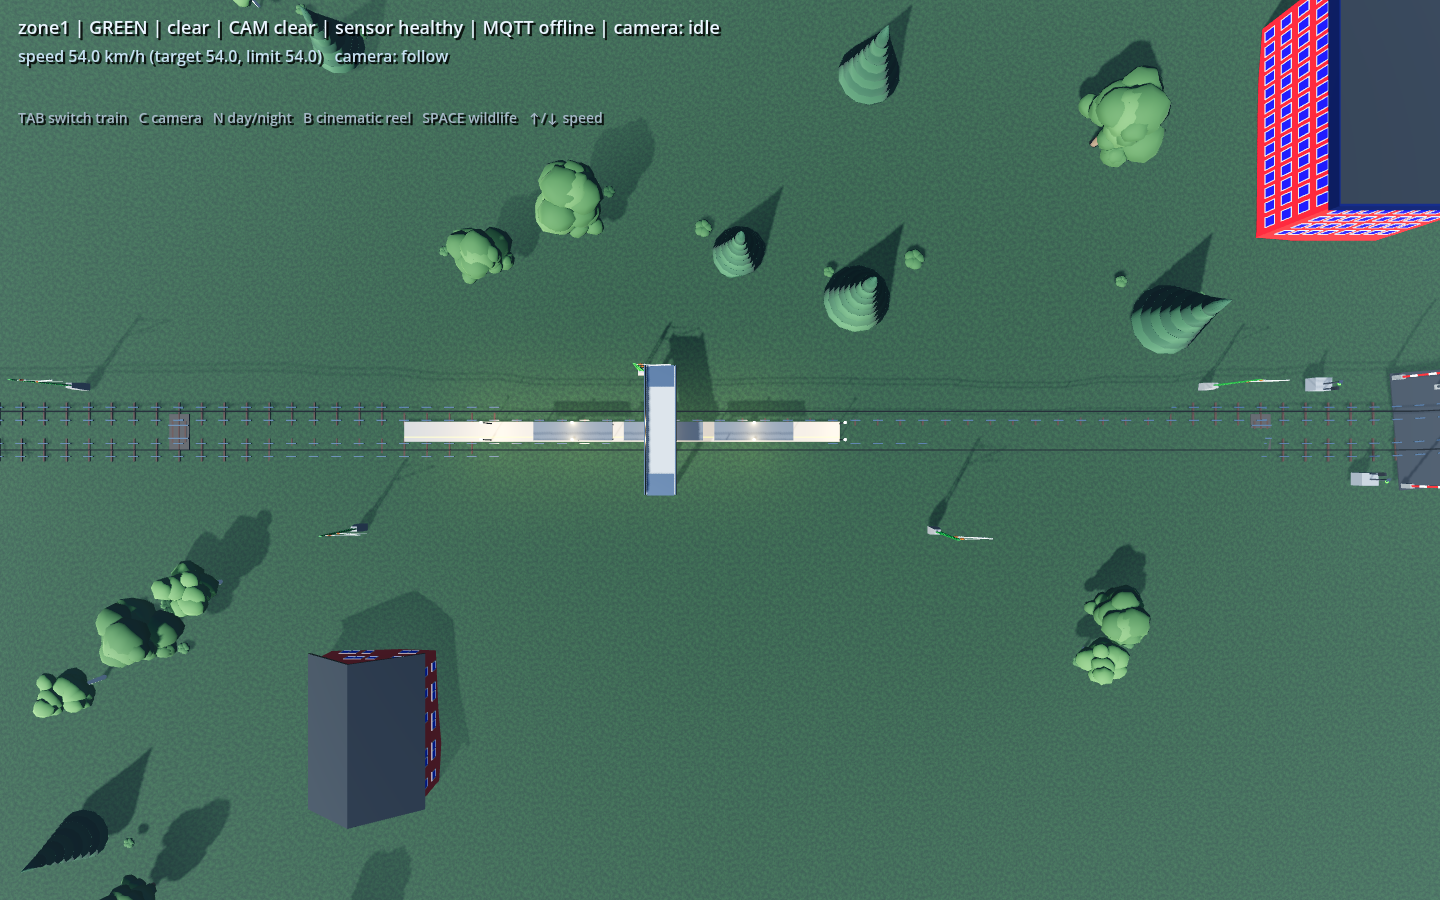
\includegraphics[width=15.2cm]{platform_after_topdown.png}
\caption{Island station between UP/DOWN tracks (top-down).}
\label{fig:plf}
\end{figure*}

\begin{figure*}\centering
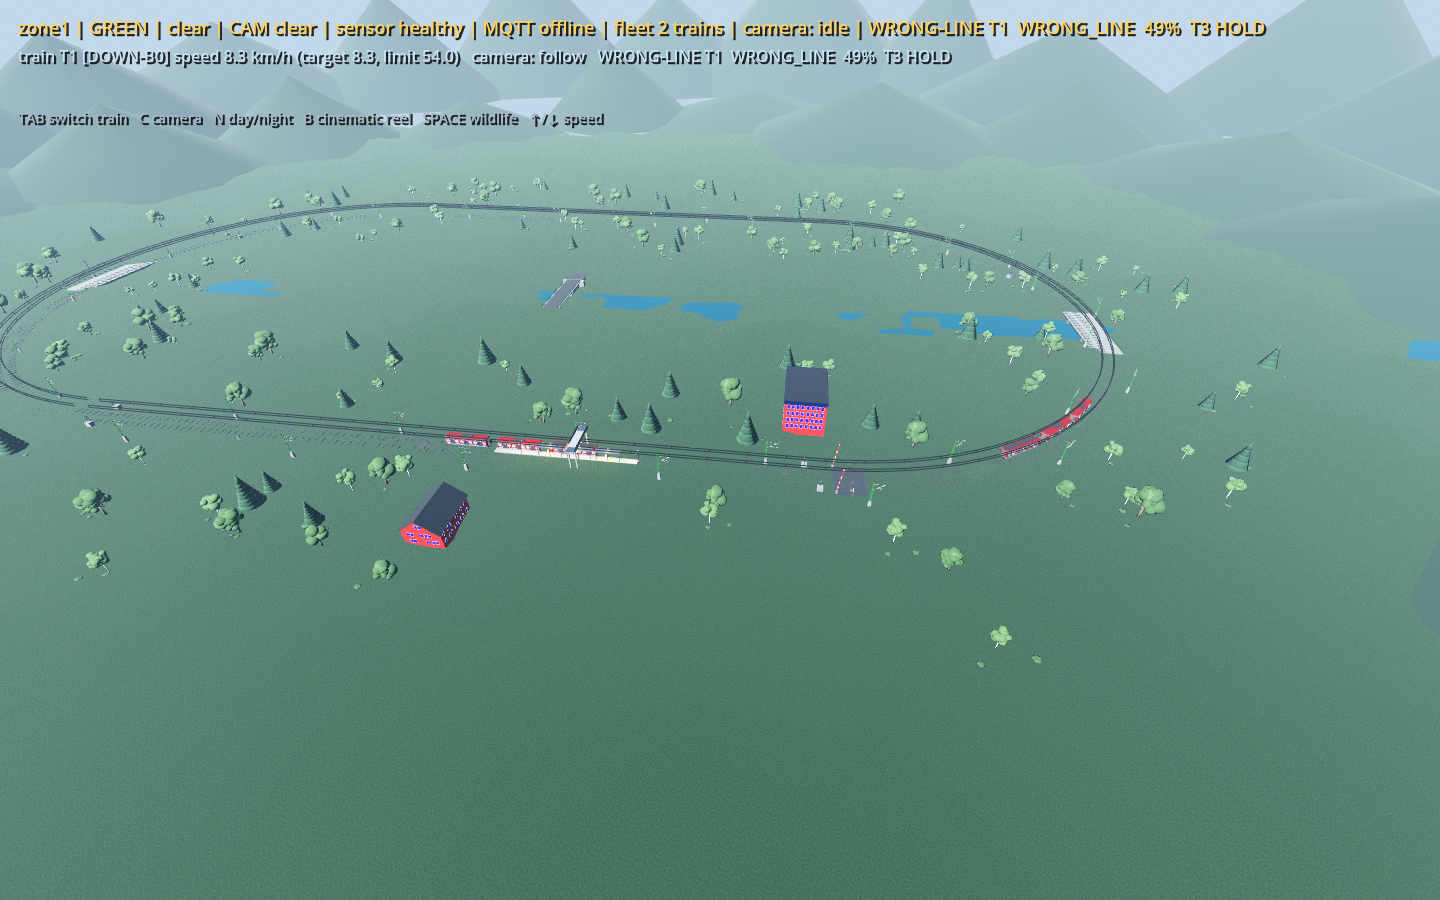
\includegraphics[width=15.2cm]{wrong_line_midway.png}
\caption{Interlocked wrong-line run: train blended onto the DOWN line at crossover A.}
\label{fig:wl}
\end{figure*}

% ================= 8. DASHBOARDS =================
\sect{VIII. Dashboards}
\textbf{Web dashboard} (\texttt{web/src/App.tsx}): login with role-aware affordances (viewer observes; operator controls; admin inspects audit --- enforced again server-side); top bar with MQTT pill and clock; hero actions (inject wildlife, simulate fault); fleet grid of per-train cards (current/target speed, occupied block, UP/DOWN pill, clockwise/anticlockwise); \textbf{Station Hold Scheduler} meet card (seed, phase, holder, route, countdown); \textbf{Wrong-Line Run} operator panel (eligibility, start, cancel; note ``X-A entry / X-B exit'' with opposing-train hold); \textbf{Sensor $\rightarrow$ Camera $\rightarrow$ Stop} wildlife panel (stage NONE/SUSPECTED/CONFIRMED, evidence sources, confidence, species, camera ONLINE/DEGRADED, ML STUB/LOADED, 30\,km/h near warning); \textbf{block signalling \& occupancy} diagram with per-block aspects and CAM/HUT evidence badges; \textbf{Audit \& Operations Log} live event stream; \textbf{Wokwi ESP32} health card. \textbf{Twin-side HUD} mirrors the same backend state (zone, aspect, CAM state and confidence, sensor health, MQTT flag, speed/target/limit, meet and wrong-line HUD, camera-capture HUD in Fig.~\ref{fig:cam}). Diagnostics: \texttt{GET /api/health} (\texttt{\{"ok":true,"mqttConnected":true\}}), \texttt{docker compose logs mqtt} for ACL denials, admin audit inspection.

% ================= 9. FEATURES =================
\sect{IX. Features and Functions Implemented}
\begin{table}[H]\scriptsize
\caption{Feature inventory with verification evidence}\label{tab:feat}
\begin{tabularx}{\linewidth}{p{3.35cm} X}
\toprule
\textbf{Feature} & \textbf{Implementation / evidence}\\
\midrule
Auth + RBAC + audit & bcrypt/JWT login; viewer/operator/admin; audit row on every accepted/rejected/forbidden attempt (\texttt{auth/rbac/audit.js}; \texttt{auth.test.js})\\
Envelope anti-replay & schema + $\pm$5\,min freshness + persistent \texttt{processed\_requests} registry (\texttt{validate/replay.js})\\
COMMS fail-safe & \texttt{COMM\_LOST} state + retained reconcile + recovery latch requiring explicit RESET\\
Two-train fleet + 10 blocks & occupancy safety (never onto RED; own-overlap allowance), per-block aspects, retained signals (\texttt{signalling.test.js}, \texttt{simulation.test.js})\\
Crossover interlock & one route at a time, hazard/occupancy 409s, audited \texttt{route:set} (\texttt{routes.test.js})\\
Seeded meets & PRNG-reproducible hold + route execution (\texttt{meets/rng.test.js})\\
Wrong-line run & phases APPROACH$\rightarrow$CROSS\_ENTRY$\rightarrow$WRONG\_LINE$\rightarrow$CROSS\_EXIT$\rightarrow$CLEARANCE$\rightarrow$DONE; opponent auto-held inside braking distance (live: T3 settled 320.1\,m)\\
Distributed huts & 10 huts, 75\,m radius, status lamps, \texttt{railway/wildlife} observations (\texttt{test\_sensor\_huts})\\
Onboard camera & forward cone $\pm$25$^\circ$/10$^\circ$, 180--200\,m, analytic occlusion (terrain/trunks/decks), confidence scoring (\texttt{test\_onboard\_detector})\\
Stopping-distance model & $d=v\,t_r+v^2/2a+d_m$ (56\,m at 36\,km/h), safe-speed inversion (\texttt{test\_onboard\_braking})\\
Staged hazard chain & trackside-only $\rightarrow$ SUSPECTED/YELLOW/30\,km/h; two-frame camera confirm $\rightarrow$ CONFIRMED/RED/0\,km/h; clear never downgrades; ESP32 \texttt{NEAR}/\texttt{DETECTED} delivery (\texttt{near\_animal.test.js} 9/9, \texttt{camera.test.js} 9/9)\\
Camera ingest guards & bearer token, \texttt{X-Captured-At} freshness, \texttt{X-Block} targeting, duplicate-id suppression, 413 oversize, 429 rate ($>$5\,fps), evidence cap 50 (\texttt{camera.test.js})\\
ESP32 edge node & restrictive-first outputs, edge-triggered \texttt{WILDLIFE\_NEAR}/\texttt{DETECTED}/\texttt{CLEARED}, zone-gated commands, buzzer pulses (16/16 native)\\
ML service & SSDLite MobileNetV3 COCO-animal detection; \texttt{ML\_STUB} deterministic elephant; edge tests: 413, 503, invalid-image rejection (8/8 pytest)\\
Legacy hole removed & anonymous \texttt{POST /api/event} deleted (404); every control authenticated + audited\\
\bottomrule
\end{tabularx}
\end{table}

% ================= 10. RESULTS =================
\sect{X. Results and Discussion}
Final automated gate \textbf{(2026-10-23 closure audit)}: backend \textbf{141/141}, Godot \textbf{42/42}, ML \textbf{8/8}, ESP32 native \textbf{16/16}, firmware build \textbf{PASS} (Flash 87.1\%), web build \textbf{PASS}. Recorded live runs: wrong-line request \texttt{WL-T1-1} held T3 at physical 320.1\,m and released only on clearance; meet seed 4242 held T3 (48$\rightarrow$0\,km/h) with \texttt{HELD} outcome and identical history on identical seeds; near$\rightarrow$confirm chain produced SUSPECTED (YELLOW, 30\,km/h limit, \texttt{WILDLIFE\_NEAR}) then CONFIRMED elephant 0.92 (RED, 0\,km/h, \texttt{WILDLIFE\_DETECTED}) with \texttt{RECOVERY\_REQUIRED} latch and operator re-arm via \texttt{/api/speed}. Gate progression: backend 84$\rightarrow$106$\rightarrow$109$\rightarrow$118$\rightarrow$137$\rightarrow$141; Godot 16$\rightarrow$22$\rightarrow$34$\rightarrow$39$\rightarrow$42; ESP32 native 14$\rightarrow$16. \textbf{Limitations:} educational only; physical-hardware checklist not run; real ML weights not exercised (stub used); capture-mode frames are seconds apart so two-frame confirmation is verified over live HTTP instead. \textbf{Conclusion:} the architecture (one authority, many restricted clients, REST commands + retained MQTT state) survived every exercised failure mode and every subsystem is gated green; remaining gaps are exercise, not architecture.

% ================= REFERENCES =================
\sect{References}
{\scriptsize
\begin{enumerate}[itemsep=0.5pt,topsep=1pt,label={[\arabic*]}]
\item Godot Engine docs, 4.x, \url{https://docs.godotengine.org/}
\item Eclipse Mosquitto 2 docs, \url{https://mosquitto.org/}
\item OASIS, MQTT Version 5.0 Specification, 2019.
\item HiveMQ, ``MQTT Essentials'' series (retained messages, QoS, topics), \url{https://www.hivemq.com/mqtt-essentials/}
\item Wokwi docs (ESP32, \texttt{diagram.json}, CLI), \url{https://docs.wokwi.com/}
\item PlatformIO docs (\texttt{platformio.ini}, Unity tests), \url{https://docs.platformio.org/}
\item D. Hardt et al., ``JSON Web Token Best Current Practices,'' RFC~8725, IETF, 2020.
\item A. Howard et al., ``Searching for MobileNetV3,'' ICCV 2019, pp.~1314--1324 (torchvision \texttt{ssdlite320\_mobilenet\_v3\_large}).
\item Express 4.x API docs, \url{https://expressjs.com/}
\item React 18 docs, \url{https://react.dev/}
\item Libre-TrainSim contributors, \url{https://github.com/JbDoe/libre-trainsim}
\item SQLite WAL-mode docs, \url{https://www.sqlite.org/wal.html}
\item FastAPI docs, \url{https://fastapi.tiangolo.com/}
\item Pinggy docs (raw TCP tunnels), \url{https://pinggy.io/docs/}
\end{enumerate}
}

\end{document}
